% 原书 p.266–p.273（PDF p.274–p.281）；第 9 章 9.6 节（三角范畴）
% 说明：本文件不含 \chapter（第 9 章标题由 ch09a 写出）。PDF p.274 顶部仍是 9.5 节的
%       收尾内容（(9.36) 与注 9.5.5），按页范围由本文件承接，之后才是 9.6 节。
% >>> p274
对于记号，正合三角中的第三个位置通常称为「锥」（cone，或「映射锥」mapping cone），
记作 $\mathrm{Cone}(\cdot)$。例如，在正合三角
$L_{k-1}\to Z_{k-1}\to L\to L_{k-1}[1]$ 中，通常写作
$L=\mathrm{Cone}(L_{k-1}\to Z_{k-1})$。类似地，
$Z_{k-1}=\mathrm{Cone}(L_{k-2}\to Z_{k-2})$。归纳地，我们可以用\textbf{迭代映射锥}
把 $L$ 与 $L'$ 联系起来：
\begin{equation}\tag{9.36}
L=\mathrm{Cone}\left(L_{k-1}\to\mathrm{Cone}(L_{k-2}\to\cdots)\cdots
\to\mathrm{Cone}(L_2\to\mathrm{Cone}(L_1\to L'))\cdots\right).
\end{equation}
在代数拓扑中，连续映射 $f:X\to Y$ 的映射锥是一种把 $X$ 从 $Y$ 中「减去」的拓扑方式。
因此 (9.36) 中的迭代映射锥大致意味着：可以由 $L$ 与 $L_1,\cdots,L_{k-1}$ 重构出
$L'$。

\begin{wrem}{9.5.5}
定理 9.5.1 中的三角范畴 $\mathcal F$ 是 $(M,\omega)$ 的 Fukaya 范畴的某个版本，记作
$\mathrm{Fuk}(M,\omega)$，它是辛几何中著名的代数结构。它提供了一种同时关联多个
拉格朗日子的同调进路，其构造主要基于拉格朗日 Floer 上同调，即第 5 章哈密顿 Floer
同调理论的相对版本。此话题超出本书范围；有兴趣的读者可参看 [201]。
\end{wrem}

% [Tutor Note: 术语依据——「锥」（cone / mapping cone）在拓扑、链复形与三角范畴三个
% 层面含义相通：拓扑上是把 $V\times[0,1]$ 的一端压成一点并沿 $f$ 粘到 $W$；链复形层面
% 就是本节 (9.38) 下方给出的矩阵微分；三角范畴层面则把「锥」抽象为三角的第三个对象。
% 记住这条线索有助于理解 9.6 节后半「为什么叫映射锥」的讨论。]

\section{三角范畴（Triangulated Category）}

\begin{keytakeaways}
\begin{itemize}
  \item 几何图像：三角范畴把「正合三角」$X\to Y\to Z\to X[1]$ 当作基本对象，
        用「与三角打交道」代替「与态射打交道」；三角的第三个位置就是映射锥。
  \item 数学工具：公理 (i)–(vi)（同构封闭、单位三角、嵌入三角、旋转、态射填充、
        八面体公理）；链复形同伦范畴 $K(\mathcal A)$ 是三角范畴的标准例子，
        其三角由映射锥构造。
  \item 本节结论：同伦范畴 $K(\mathcal A)$ 是三角范畴（定理 9.6.1）；映射锥在拓扑与
        同调代数两种意义下一致（练习 9.6.3 与 (9.39)–(9.41) 前后的讨论）。
  \item 定量工具：用「把 $Y$ 由 $X$ 经多少次映射锥搭出」定义碎片化距离
        $\delta^{F}_{\mathrm{frag}}(X,Y)$ 与配边范畴版本
        $\delta^{\mathrm{Ob}(\mathcal F)}_{\mathrm{frag}}(L,L')$，它引向范畴熵与
        三角持久范畴（TPC）。
\end{itemize}
\end{keytakeaways}

受 9.5 节末尾所示代数结构的启发，我们简要梳理三角范畴的一些基本知识。更详细的
处理见 [135] 的 1.5 节。

\begin{wdefn}{9.6.1}
称阿贝尔范畴 $\mathcal C$ 为\textbf{三角范畴}（triangulated），如果存在一个自等价
$\Sigma:\mathcal C\to\mathcal C$（通常记作 $\Sigma(\cdot)=(\cdot)[1]$），以及一族
形如 $X\to Y\to Z\to X[1]$ 的三角（称为\textbf{正合三角}（exact triangles）或
\textbf{区分三角}（distinguished triangles）），满足如下公理：
\begin{enumerate}[label=(\roman*)]
  \item 与正合三角同构的三角也是正合的（换言之，三角对三角的同构是「封闭」的）。
        更明确地说，给定正合三角 $X\to Y\to Z\to X[1]$，若另一个
        $(X',Y',Z')\cong(X,Y,Z)$ 在每一位置同构，则 $X'\to Y'\to Z'\to X'[1]$
        也正合，且下图交换。
        \[
        \begin{array}{ccccccc}
        X & \xrightarrow{f} & Y & \longrightarrow & Z & \longrightarrow & X[1]\\
        {\scriptstyle\cong}\big\downarrow & &
        {\scriptstyle\cong}\big\downarrow & &
        {\scriptstyle\cong}\big\downarrow & &
        {\scriptstyle\cong}\big\downarrow\\
        X' & \xrightarrow{f'} & Y' & \longrightarrow & Z' & \longrightarrow & X'[1]
        \end{array}
        \]
  \item 对任意 $X\in\mathrm{Ob}(\mathcal C)$，三角
        $X\xrightarrow{\mathbf 1_X}X\to0\to X[1]$ 是正合三角。
  \item 任意态射 $f:X\to Y$ 都可以嵌入一个正合三角，即存在对象 $Z$ 使得三角
        $X\xrightarrow{f}Y\to Z\to X[1]$ 正合。
  \item 三角 $X\xrightarrow{f}Y\xrightarrow{g}Z\xrightarrow{h}X[1]$ 正合，当且仅当
        其「旋转」
        $Y\xrightarrow{g}Z\xrightarrow{h}X[1]\xrightarrow{-f[1]}Y[1]$ 正合。
  \item 给定两个正合三角以及两三角中第一个态射之间的映射，则存在两三角中第三个
        对象之间的态射，使一切都交换。确切地说，给定两个三角
        $X\xrightarrow{f}Y\to Z\to X[1]$、
        $X'\xrightarrow{f'}Y'\to Z'\to X'[1]$ 以及态射 $u,v,u[1]$，存在
        $h:Z\to Z'$ 使下图交换。
        \[
        % >>> p275
        \begin{array}{ccccccc}
        X & \xrightarrow{f} & Y & \longrightarrow & Z & \longrightarrow & X[1]\\
        {\scriptstyle u}\big\downarrow & &
        {\scriptstyle v}\big\downarrow & &
        {\scriptstyle h}\big\downarrow & &
        {\scriptstyle u[1]}\big\downarrow\\
        X' & \xrightarrow{f'} & Y' & \longrightarrow & Z' & \longrightarrow & X'[1]
        \end{array}
        \]
  \item （八面体公理）给定正合三角
        $X\xrightarrow{f}Y\to Z'\to X[1]$ 与
        $Y\xrightarrow{g}Z\to X'\to Y[1]$，则存在正合三角
        $Z'\xrightarrow{h_1}Y'\xrightarrow{h_2}X'\xrightarrow{h_3}Z'[1]$，使得下图
        交换。注意 $Y'$ 的存在性来自上面的公理 (iii)，而 $h_1,h_2,h_3$ 的存在性
        来自上面的公理 (v)。
        \[
        \begin{array}{ccccccc}
        X & \xrightarrow{f} & Y & \longrightarrow & Z' & \longrightarrow & X[1]\\
        {\scriptstyle\mathbf 1_X}\big\downarrow & &
        {\scriptstyle g}\big\downarrow & &
        {\scriptstyle h_1}\big\downarrow & &
        {\scriptstyle\mathbf 1_{X[1]}}\big\downarrow\\
        X & \xrightarrow{g\circ f} & Z & \longrightarrow & Y' & \longrightarrow & X[1]\\
        \big\downarrow & & \big\downarrow & &
        {\scriptstyle h_2}\big\downarrow & & \big\downarrow\\
        0 & \longrightarrow & X' & \xrightarrow{\mathbf 1_{X'}} & X' & \longrightarrow & 0\\
        \big\downarrow & & \big\downarrow & &
        {\scriptstyle h_3}\big\downarrow & & \big\downarrow\\
        X[1] & \longrightarrow & Y[1] & \longrightarrow & Z'[1] & \longrightarrow & X[2]
        \end{array}
        \]
\end{enumerate}
\end{wdefn}

% [Tutor Note: 易错预警——这些公理是三角范畴的常见版本，但各文献编号与强弱略有差异：
% (i) 通常并入 TR1（三角类对同构封闭），(ii)(iii) 属于 TR1，(iv) 是 TR2（旋转），
% (v) 是 TR3（态射填充），(vi) 是 TR4（八面体公理）。引用时请注明所依据的文献
% （如 Weibel《An Introduction to Homological Algebra》第 10 章、Neeman《Triangulated
% Categories》）。另注意 (iv) 中旋转的符号是 $-f[1]$：这个负号是符号约定的关键，
% 写成 $+f[1]$ 会导致与链复形例子 (9.38) 的符号不一致。]

\begin{wrem}{9.6.1}
在正合三角 $X\xrightarrow{f}Y\xrightarrow{g}Z\xrightarrow{h}X[1]$ 中，第三个位置
通常称为态射 $f:X\to Y$ 的\textbf{映射锥}（mapping cone，cf.\ 例 9.6.2）。因此，
定义 9.6.1 中的公理 (vi) 通常被记忆为「复合的映射锥是映射锥的映射锥」（up to 公理
(iv) 中的三角旋转）。
\end{wrem}

% [Tutor Note: 含糊点拨——八面体公理 (vi) 是六条公理中最不直观的一条。把它读成
% 「(6) 的交换图 + 逐行/逐列的正合三角」即可：每一行、每一列都是一个正合三角，
% 且中间一行的第一个对象是 $g\circ f$。它的实质是保证「映射锥的映射锥」与
% 「复合的映射锥」在三角意义下只差一次旋转。若读者只关心 Biran–Cornea 构造，
% 可先接受此公理，重点记住 9.6 节末尾「用映射锥把大空间切成小块并数次数」的
% 定量用法。]

我们已经看到定义 9.6.1 相当复杂。然而，这是一个有趣而深刻的想法：它用「与三角
打交道」替换「与态射打交道」。后者更形式化，且显然更强大。下面的引理及其证明就是
一个例子。

\begin{wlem}{9.6.1}
若 $X\xrightarrow{f}Y\xrightarrow{g}Z\xrightarrow{h}X[1]$ 是正合三角，则
\[
g\circ f=h\circ g=f[1]\circ h=0.
\]
\end{wlem}

% >>> p276
\begin{wproof}
让我们证明 $g\circ f=0$。考虑如下交换图。
\[
\begin{array}{ccccccc}
X & \xrightarrow{\mathbf 1_X} & X & \xrightarrow{0} & 0 & \longrightarrow & X[1]\\
{\scriptstyle\mathbf 1_X}\big\downarrow & &
{\scriptstyle f}\big\downarrow & &
{\scriptstyle h}\big\downarrow & &
{\scriptstyle\mathbf 1_{X[1]}}\big\downarrow\\
X & \xrightarrow{f} & Y & \xrightarrow{g} & Z & \longrightarrow & X[1]
\end{array}
\]
由公理 (v)，存在 $h:0\to Z$ 使第二个方块交换。因此 $0=g\circ f$。其余结果留给有兴趣
的读者。
\end{wproof}

% [Tutor Note: 含糊点拨——「其余结果」指的是 $h\circ g=0$ 与 $f[1]\circ h=0$：对已证的
% 三角作公理 (iv) 的旋转，即可把 $g\circ f=0$ 分别翻译成 $h\circ g=0$（旋转一次）与
% $f[1]\circ h=0$（旋转两次，注意符号）。这三条是「三角是复形」的精确含义，也是
% 下一节 (9.38) 中 $\pi^\bullet\circ i^\bullet=0$ 的来源。]

\begin{wexer}{9.6.1}
(i) 设 $X\xrightarrow{f}Y\xrightarrow{g}Z\xrightarrow{h}X[1]$ 是正合三角。对固定的
$A\in\mathrm{Ob}(\mathcal C)$，可以作用函子
$\mathrm{Hom}_{\mathcal C}(A,\cdot)$，它把 $\mathcal C$ 映到阿贝尔群范畴。证明它
诱导出如下长正合列：
\[
\cdots\to\mathrm{Hom}_{\mathcal C}(A,X)\to\mathrm{Hom}_{\mathcal C}(A,Y)
\to\mathrm{Hom}_{\mathcal C}(A,Z)\to\mathrm{Hom}_{\mathcal C}(A,X[1])\to\cdots.
\]
(ii) 证明：在下图中，若给定的态射 $f,g$ 是 $\mathcal C$ 中的同构，则由公理 (v)
诱导的态射 $h$ 也是 $\mathcal C$ 中的同构。
\[
\begin{array}{ccccccc}
X & \longrightarrow & Y & \longrightarrow & Z & \longrightarrow & X[1]\\
{\scriptstyle f}\big\downarrow & &
{\scriptstyle g}\big\downarrow & &
{\scriptstyle h}\big\downarrow & &
{\scriptstyle f[1]}\big\downarrow\\
X' & \longrightarrow & Y' & \longrightarrow & Z' & \longrightarrow & X'[1]
\end{array}
\]
\end{wexer}

% [Tutor Note: 易错预警——(i) 的要点是 $\mathrm{Hom}_{\mathcal C}(A,\cdot)$ 把正合三角
% 变为长正合列（这正是「正合三角」之名的来源）；对反变函子
% $\mathrm{Hom}_{\mathcal C}(\cdot,A)$ 也可得到长正合列，但方向相反。
% (ii) 的证明可用「五引理」或把 (i) 用于所有 $A$，再配合 Yoneda 引理。]

\begin{wexam}{9.6.1}
对任意 $x\in L_1\cap L_2$，配边 $V_x:L_1\#_x L_2\to(L_1,L_2)$ 在定理 9.5.1 中
出现的范畴 $\mathcal F$ 中诱导一个正合三角
\begin{equation}\tag{9.37}
L_2\to L_1\to L_1\#_x L_2\to L_2[1].
\end{equation}
通常写作 $L_1\#_x L_2=\mathrm{Cone}(L_2\to L_1)$。\hfill$//$
\end{wexam}

% [Tutor Note: 术语依据——$L_1\#_x L_2$ 是拉格朗日连通和（Lagrangian connected sum，
% 亦作 Lagrangian surgery），即在相交点 $x$ 处把两个拉格朗日子流形「焊」起来。
% (9.37) 是 Biran–Cornea 配边范畴中「锥 = 连通和」的精确表述；其函子性依赖于
% 定理 9.5.1 中的三角范畴 $\mathcal F$ 的构造，这正是本节讨论三角范畴的动机。]

\begin{wexam}{9.6.2}
固定一个域 $\mathbf k$，记 $\mathcal A$ 为 $\mathbf k$-模范畴。令 $C(\mathcal A)$
为\textbf{上链复形}范畴，其对象 $\mathrm{Ob}(C(\mathcal A))$ 是序列
\[
(C^\bullet,d_C)=
\left(\cdots\to C^{-1}\xrightarrow{d_C^{-1}}C^0
\xrightarrow{d_C^0}C^1\xrightarrow{d_C^1}\cdots\right).
\]
Hom-集 $\mathrm{Mor}_{C(\mathcal A)}((C^\bullet,d_C),(D^\bullet,d_D))$ 由满足如下
交换图的一族态射 $f^\bullet=\{f^k:C^k\to D^k\}_{k\in\Z}$ 组成。
\[
\begin{array}{ccccccc}
\cdots & \longrightarrow & C^0 & \xrightarrow{d_C^0} & C^1 & \longrightarrow & \cdots\\
& & {\scriptstyle f^0}\big\downarrow & & {\scriptstyle f^1}\big\downarrow & & \\
\cdots & \longrightarrow & D^0 & \xrightarrow{d_D^0} & D^1 & \longrightarrow & \cdots
\end{array}
\]
\hfill$//$
\end{wexam}

% >>> p277
迄今为止，范畴 $C(\mathcal A)$ 上几乎没有结构。我们如下修改 $C(\mathcal A)$：
对任意 $f^\bullet,g^\bullet\in
\mathrm{Mor}_{C(\mathcal A)}((C^\bullet,d_C),(D^\bullet,d_D))$，若 $f^\bullet$ 与
$g^\bullet$ 之间存在链同伦，则定义 $f^\bullet\sim g^\bullet$。换言之，存在
$h^\bullet=\{h^k:C^k\to D^{k-1}\}_{k\in\Z}$ 使下图交换，其中
$f^k-g^k=h^{k+1}\circ d_C^k+d_D^{k-1}\circ h^k$。注意在上同调群层面，两个链同伦
的映射 $f$ 与 $g$ 诱导同一个映射，即
$f_*=g_*:H^*(C^\bullet,d_C)\to H^*(D^\bullet,d_D)$。类似地，可以定义两个上链复形
之间的同伦等价关系。
\[
\begin{array}{ccccccccc}
\cdots & \longrightarrow & C^{-1} & \longrightarrow & C^0 & \xrightarrow{d_C^0} & C^1
& \longrightarrow & \cdots\\
& & \big\downarrow & \overset{\scriptstyle h^0}{\swarrow} & \big\downarrow
& \overset{\scriptstyle h^1}{\swarrow} & \big\downarrow & & \\
\cdots & \longrightarrow & D^{-1} & \xrightarrow{d_D^{-1}} & D^0 & \longrightarrow & D^1
& \longrightarrow & \cdots
\end{array}
\]
现在考虑由下式定义的 $\mathbf k$-模的\textbf{同伦范畴}
\[
K(\mathcal A):=C(\mathcal A)\big/\sim\ =
\begin{cases}
\mathrm{Ob}(K(\mathcal A))=\mathrm{Ob}(C(\mathcal A)),\\[2pt]
\mathrm{Mor}_{K(\mathcal A)}((C^\bullet,d_C),(D^\bullet,d_D))
=\mathrm{Mor}_{C(\mathcal A)}((C^\bullet,d_C),(D^\bullet,d_D))\big/\sim,
\end{cases}
\]
其中 $\sim$ 是同伦关系。于是我们有如下关键性质：

\begin{wthm}{9.6.1}
同伦范畴 $K(\mathcal A)$ 是三角范畴。
\end{wthm}

\begin{wproof}
定义 $\Sigma:C(\mathcal A)\to C(\mathcal A)$ 为平移次数的函子，即在对象层面
$\Sigma((C^\bullet,d_{C^\bullet})):=(C^{\bullet+1},d_{C^\bullet+1})$。我们将定义
一族三角，并把它们标为正合三角（然后验证这些正合三角满足定义 9.6.1 中所需的公理）。

正合三角将取为与如下三角同构的三角：
\begin{equation}\tag{9.38}
C^\bullet\xrightarrow{f^\bullet}D^\bullet\xrightarrow{i^\bullet}
\mathrm{Cone}(f)^\bullet\xrightarrow{\pi^\bullet}C^\bullet[1],
\end{equation}
其中 $\mathrm{Cone}(f)^\bullet$ 是 $f^\bullet$ 的映射锥。下面是此设定中映射锥的
显式定义。

作为上链复形，$\mathrm{Cone}(f)^k=C^{k+1}\oplus D^k$，其微分
$d_{\mathrm{co}}^k:C^{k+1}\oplus D^k\to C^{k+2}\oplus D^{k+1}$ 由如下矩阵给出：
\[
d_{\mathrm{co}}^k\begin{pmatrix}c<本地路径>
=\begin{pmatrix}d_C^{k+1}&0\\ f^{k+1}&d_D^k\end{pmatrix}
\begin{pmatrix}c<本地路径>
=\begin{pmatrix}d_C^{k+1}(c)\\ f^{k+1}(c)+d_D^k(d)\end{pmatrix},
\]
其中 $d_C^{k+1}(c)\in C_{k+2}$、$f^{k+1}(c)+d_D^k(d)\in D_{k+1}$。此外在 (9.38)
中，映射 $i^\bullet:D^\bullet\to\mathrm{Cone}(f)^\bullet$ 是第二个因子的嵌入；
$\pi^\bullet:\mathrm{Cone}(f)^\bullet\to C^\bullet[1]$ 是到第一个因子的投影。论证的
其余部分由繁琐的验证组成（见 [135] 的 1.4 节）。
\end{wproof}

% [Tutor Note: 原文疑误——「其中 $d_C^{k+1}(c)\in C_{k+2}$、$f^{k+1}(c)+d_D^k(d)\in
% D_{k+1}$」中的上链复形应带\emph{上}指标，即 $C^{k+2}$ 与 $D^{k+1}$；原文印成
% 下指标（$C_{k+2}$、$D_{k+1}$），与本节通篇的上链记号矛盾。译文照原文保留并在此
% 说明，已记入 review_ch09b.md。]

% [Tutor Note: 易错预警——映射锥微分的矩阵约定各家不同：本书用
% $\begin{pmatrix}d_C&0\\ f&d_D\end{pmatrix}$（第二行是 $+f$），于是
% $d_{\mathrm{co}}^2=0$ 等价于 $f$ 是链映射（$d_D f=f d_C$）。若改用
% $\begin{pmatrix}d_C&0\\ -f&d_D\end{pmatrix}$，则 (9.38) 中 $i^\bullet$ 的符号也要相应
% 调整，否则三角不正合。核对时务必把符号约定与 (9.38) 一起看。]

\begin{wexer}{9.6.2}
（更多细节见 [28] 的 2.5.2 节）考虑\textbf{过滤链复形}范畴：其对象是三元组
$(C_\bullet,\partial_C,\ell_C)$，其中 $(C_\bullet,\partial_C)$ 是链复形，$\ell_C$
是过滤函数（见 8.2 节），满足对任意 $x\in C_\bullet$ 有
$\ell_C(\partial_C(x))\leqslant\ell_C(x)$；态射是\textbf{过滤态射}
$f_\bullet:(C_\bullet,\partial_C,\ell_C)\to(D_\bullet,\partial_D,\ell_D)$，即满足
对任意 $x\in C_\bullet$ 有 $\ell_D(f(x))\leqslant\ell_C(x)$ 的链映射。类似例 9.6.2
中的同伦范畴，可以构造\textbf{过滤同伦范畴}。然后证明所得的过滤同伦范畴（作为过滤
链复形范畴的商范畴）也是三角的，其中所有态射都保过滤。
\end{wexer}

% >>> p278
人们可能会好奇：(9.38) 中的 $\mathrm{Cone}(f)^\bullet$ 为什么叫映射锥？事实上，这里
的「映射锥」（在同调意义下）正是受代数拓扑中（拓扑）映射锥这一术语的启发。

回忆一下：给定两个拓扑空间 $V,W$ 与连续映射 $f:V\to W$，拓扑映射锥
$\mathrm{Cone}(f)$ 定义为映射柱 $(V\times[0,1])\sqcup_f W$ 的商空间，其中由记号
$\sqcup_f$ 表示的等价关系（或沿 $f$ 的粘合）由下式给出
\[
(x,0)\sim(x',0)\quad\text{且}\quad(x,1)\sim f(x)
\qquad\text{对任意 }x,x'\in V.
\]
换言之，在 $t=0$ 处所有点被压成单个点，而在 $t=1$ 处沿映射 $f$ 把 $V$ 粘到 $W$ 上。
示意图见图 9.18。从图中可以立即看出：取 $f:V\to W$ 的（拓扑）映射锥这一操作，就是
把像 $f(V)$ 从 $W$ 中「减去」。

\begin{figure}[htbp]
  \centering
  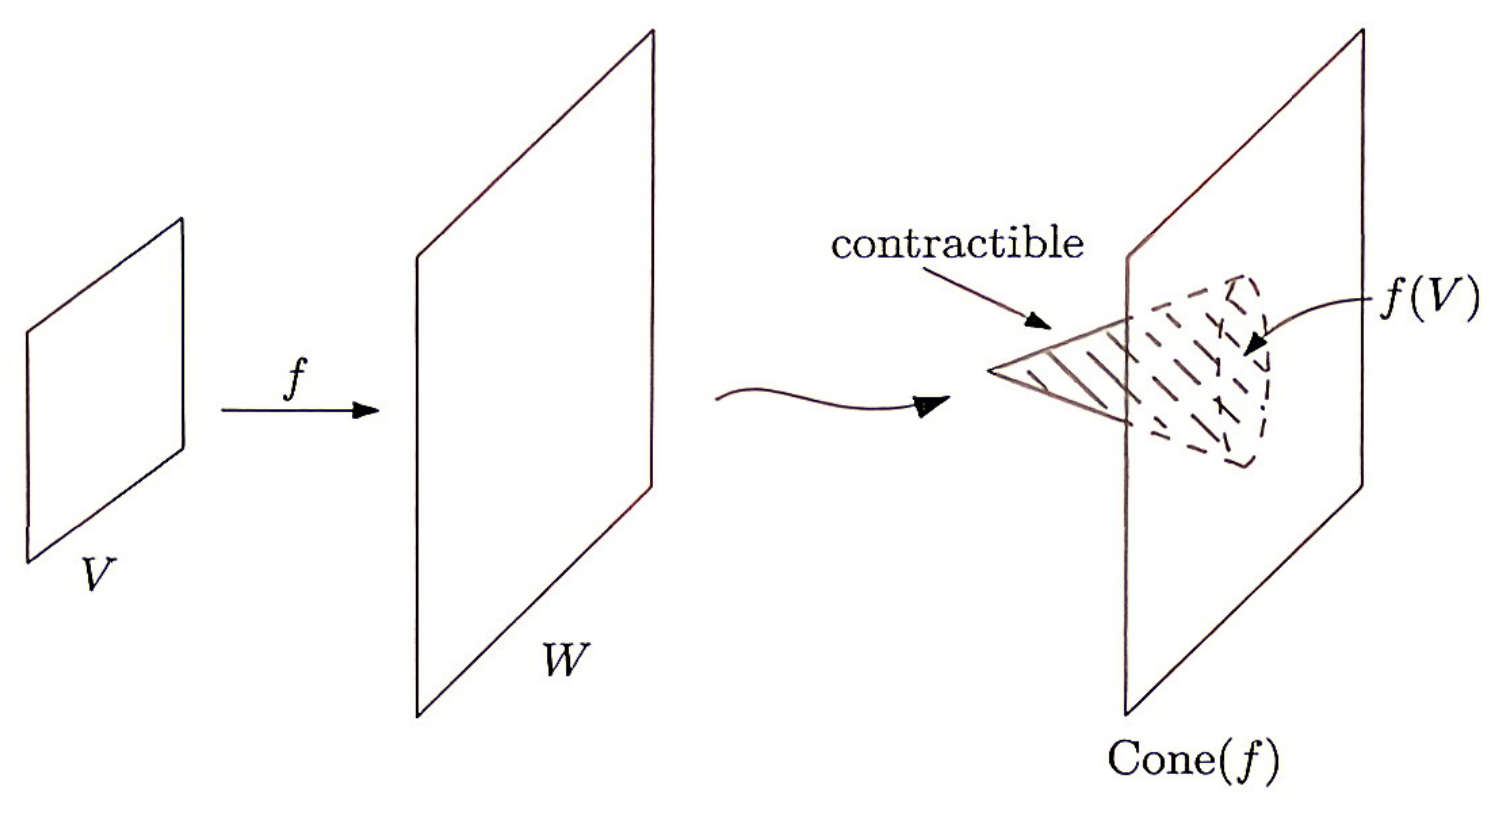
\includegraphics[width=0.72\linewidth]{figures/fig_p278_1.png}
  \caption*{图 9.18\quad $f:V\to W$ 的拓扑映射锥（原书 p.270, Figure 9.18；
  PDF p.278）}
\end{figure}

考虑图 9.19 所示的 $\mathrm{Cone}(f)$ 内部的两个开子集 $U_1$ 与 $U_2$。我们知道
$U_1\cup U_2=\mathrm{Cone}(f)$，且 $U_1\cap U_2$ 同伦等价于 $V$。于是可以对
$\Z/2\Z$ 系数应用约化奇异上链复形，得到如下短正合列：
\begin{equation}\tag{9.39}
0\to C^\bullet(U_1+U_2)\to C^\bullet(U_1)\oplus C^\bullet(U_2)
\to C^\bullet(U_1\cap U_2)\to0.
\end{equation}

% >>> p279
其中 $C^\bullet(U_1+U_2)$ 是 $C_\bullet(U_1+U_2)$ 的对偶。回忆 $C_\bullet(U_1+U_2)$
由所有可以写成 $U_1$ 中链与 $U_2$ 中链之和的链组成。

\begin{figure}[htbp]
  \centering
  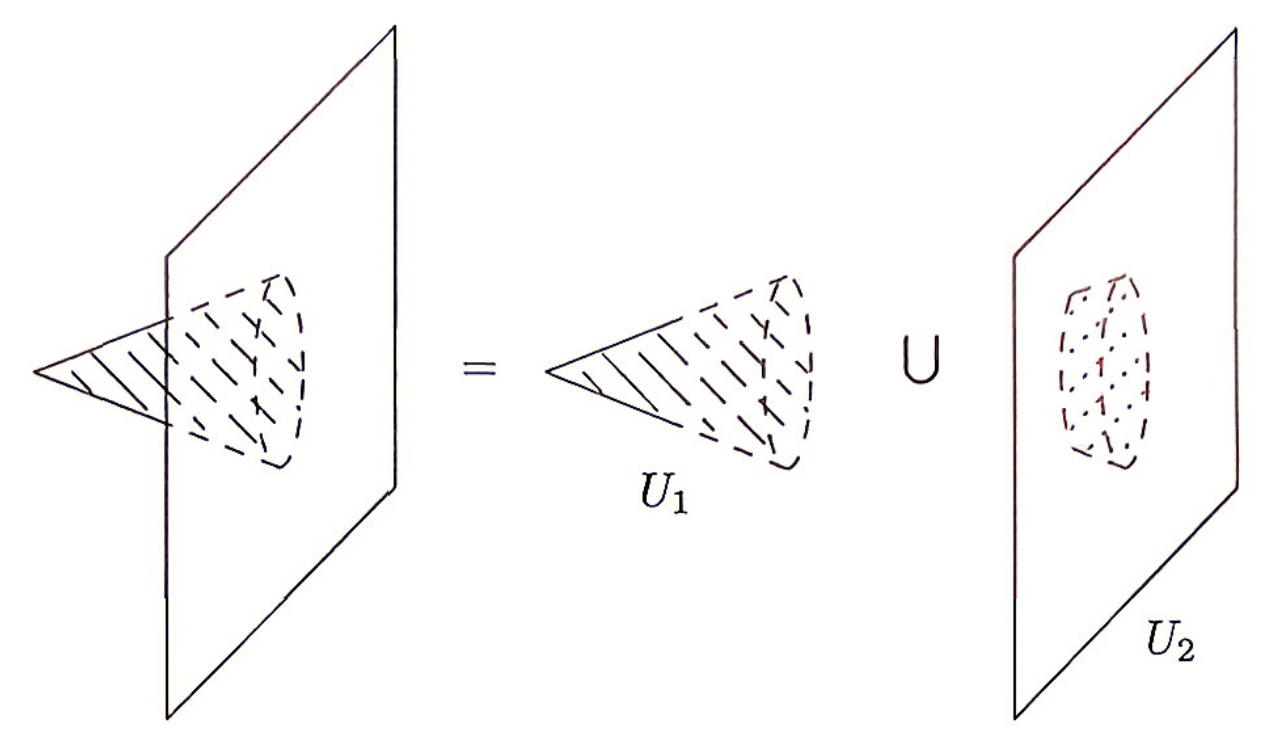
\includegraphics[width=0.62\linewidth]{figures/fig_p279_1.png}
  \caption*{图 9.19\quad 拓扑映射锥的一个开覆盖（原书 p.271, Figure 9.19；
  PDF p.279）}
\end{figure}

观察到包含映射 $i:C_\bullet(U_1+U_2)\to C_\bullet(\mathrm{Cone}(f))$ 在同调上诱导
同构，因此 $C^\bullet(\mathrm{Cone}(f))\cong C^\bullet(U_1+U_2)$。于是 (9.39) 在
同伦等价意义下给出如下短正合列
\[
0\to C^\bullet(\mathrm{Cone}(f))\to C^\bullet(W)
\xrightarrow{f^*}\to C^\bullet(V)\to0,
\]
其中 $C^\bullet(W)\cong C^\bullet(U_1)\oplus C^\bullet(U_2)$，
$C^\bullet(V)\cong C^\bullet(U_1\cap U_2)$，而 $f^*$ 由连续映射 $f$ 诱导。下面这个
练习是同调代数中的一个巧妙事实。

\begin{wexer}{9.6.3}
考虑例 9.6.2 中的同伦范畴 $K(\mathcal A)$（它由上链复形范畴 $C(\mathcal A)$
构造）。若 $0\to C^\bullet\xrightarrow{f^\bullet}D^\bullet\to E^\bullet\to0$ 是
$C(\mathcal A)$ 中上链复形的短正合列，证明 $E^\bullet$ 同伦等价于
$f^\bullet:C^\bullet\xrightarrow{f^\bullet}D^\bullet$ 在 $C(\mathcal A)$ 中的映射锥，
即
\[
E^\bullet\simeq\mathrm{Cone}(f)^\bullet\quad\text{在 }K(\mathcal A)\text{ 中}.
\]
特别地，$C(\mathcal A)$ 中的短正合列在 $K(\mathcal A)$ 中诱导正合三角
$C^\bullet\xrightarrow{f^\bullet}D^\bullet\to E^\bullet\to C^\bullet[1]$。
\end{wexer}

% [Tutor Note: 含糊点拨——练习 9.6.3 的证明是对短正合列
% $0\to C^\bullet\to D^\bullet\to E^\bullet\to0$ 作「锥的锥」：先构造
% $\mathrm{Cone}(f)^\bullet\to E^\bullet$ 的链映射（由蛇引理或五引理），再证明其在
% 同伦范畴中可逆。这条事实把「同调代数的短正合列」与「三角范畴的正合三角」对应
% 起来，是 (9.38) 之后一切论证的基础。]

于是由上面的练习 9.6.3，
\[
\mathrm{Cone}(f)\left(=\mathrm{Cone}(f:V\to W)\right)
=\mathrm{Cone}\left(f^\bullet:C^\bullet(W)\to C^\bullet(V)\right).
\]
因此，两种涉及映射锥的表述彼此一致。

一般说来，从三角范畴中提取数值数据并非易事。映射锥提供了一种方式（在拓扑与同调
代数中都是如此），把大空间「切」成小空间。换言之，在三角范畴中，人们
% >>> p280
可以通过正合三角由小块恢复整个/原来的空间。循此思路，我们可以通过计算需要用多少个
正合三角，来构造一个度量此恢复过程复杂性的整值量。确切地说，对
$X,Y\in\mathrm{Ob}(\mathcal C)$，用如下量定义它们的「距离」（从 $X$ 到 $Y$）：
\begin{equation}\tag{9.40}
\delta^{F}_{\mathrm{frag}}(X,Y)
=\inf\left\{k\in\N\ \middle|\
\begin{array}{l}
\exists Z_1,\cdots,Z_{k-1}\in\mathrm{Ob}(\mathcal C)\ \text{使得}\\
Y\to0\to Z_1\to Y[1]\\
E_2\to Z_1\to Z_2\to E_2[1]\\
\cdots\\
E_{k-2}\to Z_{k-2}\to Z_{k-1}\to E_{k-2}[1]\\
E_{k-1}\to Z_{k-1}\to X\to E_{k-1}[1]\\
\text{其中}\ E_i\in F,\ 2\leqslant i\leqslant k-1
\end{array}\right\},
\end{equation}
其中 $F$ 是固定的子集 $F\subset\mathrm{Ob}(\mathcal C)$。换言之，
$\delta^{F}_{\mathrm{frag}}(X,Y)$ 度量的是：通过 $F$ 中的元素、用迭代映射锥把 $Y$
从 $X$ 搭起来所需的最少步数。

下面是一个初等的计算例子。

\begin{wexam}{9.6.3}
在 $\mathbf k$-模的同伦范畴 $K(\mathcal A)$ 中，取 $F=\{\mathbf k\}$，其中
$\mathbf k$ 表示只在次数 $0$ 处集中了一个一维 $\mathbf k$-模、其余各项全为零的上链
复形。那么 (9.40) 中仅有的正合三角就是由短正合序列（由练习 9.6.3）诱导的那些：
\[
0\to\mathbf k\to C^\bullet\to C^\bullet/\mathbf k\to0.
\]
这说明
\[
\delta^{F}_{\mathrm{frag}}(0,C^\bullet)
=\sum_{k=0}^{\infty}\dim_{\mathbf k}(C^k),
\]
于是我们可以显式地计算 $0$ 与 $C^\bullet$ 之间的「距离」。\hfill$//$
\end{wexam}

% [Tutor Note: 易错预警——(9.40) 中 $\inf$ 的指标 $k$ 是「正合三角的个数 + 1」，
% 且 $k=1$ 时 $\exists Z_1,\cdots,Z_{0}$ 为空条件；此外 $F$ 的选取直接影响
% $\delta^{F}_{\mathrm{frag}}$ 的取值（原文紧接着指出这一点）。例 9.6.3 中
% 「距离 = 各阶 Betti 数之和」是 (9.40) 的试金石：它说明此量确实在数「用 $\mathbf k$
% 作积木搭出 $C^\bullet$ 的步数」。]

\begin{wrem}{9.6.2}
(9.40) 中的这种量（及其在各种设定下的变体）已在 [66] 中被系统地研究，它引出一个
三角范畴中的动力系统概念，称为\textbf{范畴熵}（categorical entropy）。这是把动力
系统与范畴论结合起来的最早的成功尝试之一。
\end{wrem}

\begin{wrem}{9.6.3}
定理 9.5.1 中相继的三角与上面 (9.40) 中 $\delta^{F}_{\mathrm{frag}}(X,Y)$ 的定义
之间的相似性提示：可以定义一个量来度量配边范畴 $\mathrm{Cob}(M)$ 中两个对象（拉格朗日
子流形）之间的距离。确切地说，
\begin{equation}\tag{9.41}
\delta^{\mathrm{Ob}(\mathcal F)}_{\mathrm{frag}}(L,L')
:=\inf\left\{
\begin{array}{l}
\#\ \text{of exact triangles of}\ \Phi(V)\ \text{in}\ \mathcal F\\
\text{for cobordism}\ V\in\mathrm{Mor}_{\mathrm{Cob}(M)}(L,L')
\end{array}\right\}.
\end{equation}
\end{wrem}

% >>> p281
其中范畴 $\mathcal F$ 与函子 $\Phi$ 来自定理 9.5.1。实践中，人们通常考虑对象集的
较小真子集 $F\subset\mathrm{Ob}(\mathcal F)$，而不是整个对象集
$\mathrm{Ob}(\mathcal F)$。值 $\delta^{F}_{\mathrm{frag}}(\cdot,\cdot)$ 对 $F$ 的
选取是敏感的。

在结束本节之前，让我们指出 (9.41) 中的量
$\delta^{\mathrm{Ob}(\mathcal F)}_{\mathrm{frag}}(\cdot,\cdot)$ 会丢失一些信息。
例如，通过定义 9.5.1 中的\textbf{拉格朗日悬置}
$S(L,\{\varphi^t_H\}_{t\in\R})$（作为从 $\varphi^1_H(L)$ 到 $L$ 的拉格朗日配边），
可以得到定理 9.5.1 所示范畴 $\mathcal F$ 中的正合三角
\[
L\to0\to\varphi^1_H(L)\to L[1].
\]
因此按定义，$\delta^{\mathrm{Ob}(\mathcal F)}_{\mathrm{frag}}(L,\varphi^1_H(L))=1$。
然而，那个奇特的量——投影
$\pi(S(L,\{\varphi^t_H\}_{t\in\R}))\subset\R^2$ 的面积，即「阴影」（shadow）——
却被 $\delta^{\mathrm{Ob}(\mathcal F)}_{\mathrm{frag}}$ 完全忽略了。为了把这一几何量
编码进去，我们需要一套新的机器，称为\textbf{三角持久范畴}（triangulated
persistence category，简称 TPC），它把本节阐述的三角结构与 5.2 节阐述的持久模
结构结合起来。关于此课题的详细发展，见 [26-28]。

% [Tutor Note: 术语依据——「拉格朗日悬置」（Lagrangian suspension）$S(L,\{\varphi^t_H\})$
% 是 Biran–Cornea 构造中的基本配边：把 $L$ 沿哈密顿同痕扫过得到（$2n$ 维）拉格朗日
% 配边，其「阴影」是投影到 $\R^2$ 的面积。注 9.6.3 与 p.281 这段说明：三角结构
% 只记录「有多少个三角」，而 TPC 还要记录「面积/过滤」这种连续信息——这正是
% 第 5 章持续模思想在配边范畴中的推广（[26-28]）。]

% [Tutor Note: 含糊点拨——本节的「函子性」要点：定理 9.5.1 给出从配边范畴
% $\mathrm{Cob}(M)$ 到三角范畴 $\mathcal F$ 的函子 $\Phi$；$\delta^{\mathrm{Ob}(\mathcal F)}_{\mathrm{frag}}$
% 之所以能作为 $L,L'$ 的不变量，依赖的正是 $\Phi$ 把配边（对象间态射）送到正合三角
% （$\mathcal F$ 中对象间的三角）。若 $\Phi$ 只是「逐对象」的对应而非函子，则 (9.41)
% 中的 inf 将失去不变性。]
